\documentclass[a4paper, 11pt, notitlepage, english]{article}

\usepackage{babel}
\usepackage[utf8]{inputenc}
\usepackage[T1]{fontenc, url}
\usepackage{textcomp}
\usepackage{amsmath, amssymb}
\usepackage{amsbsy, amsfonts}
\usepackage{graphicx, color, xcolor}
\usepackage{verbatim, listings, fancyvrb}
\usepackage{parskip}
\usepackage{framed}
\usepackage{amsmath}
\usepackage{multicol}
\usepackage{url}
\usepackage{flafter}
\usepackage{simplewick}
\usepackage{amsthm}
\usepackage{bbold}


\usepackage{caption}
\DeclareCaptionLabelSeparator{colon}{. }
\renewcommand{\captionfont}{\small\sffamily}
\renewcommand{\captionlabelfont}{\bf\sffamily}
\usepackage{float}
%\floatstyle{ruled}
%\restylefloat{figure}
\setlength{\captionmargin}{20pt}
%\addto\captionsenglish{\renewcommand{\figurename}{Fig.}}
\usepackage{bigstrut}
\setlength{\tabcolsep}{12pt}


\newtheorem{theorem}[]{Wick's Theorem}[]

\DeclareUnicodeCharacter{00A0}{~}

\definecolor{javared}{rgb}{0.6,0,0} % for strings
\definecolor{javagreen}{rgb}{0.25,0.5,0.35} % comments
\definecolor{javapurple}{rgb}{0.5,0,0.35} % keywords
\definecolor{javadocblue}{rgb}{0.25,0.35,0.75} % javadoc

\lstset{language=python,
basicstyle=\ttfamily\scriptsize,
keywordstyle=\color{javapurple},%\bfseries,
stringstyle=\color{javared},
commentstyle=\color{javagreen},
morecomment=[s][\color{javadocblue}]{/**}{*/},
morekeywords={super, with},
% numbers=left,
% numberstyle=\tiny\color{black},
stepnumber=2,
numbersep=10pt,
tabsize=2,
showspaces=false,
captionpos=b,
showstringspaces=false,
frame= single,
breaklines=true}

\usepackage{geometry}
\geometry{headheight=0.01mm}
\geometry{top=20mm, bottom=20mm, left=34mm, right=34mm}

\renewcommand{\arraystretch}{2}
\setlength{\tabcolsep}{10pt}
\makeatletter
\renewcommand*\env@matrix[1][*\c@MaxMatrixCols c]{%
  \hskip -\arraycolsep
  \let\@ifnextchar\new@ifnextchar
  \array{#1}}
%
% Definering av egne kommandoer og miljøer
%
\newcommand{\dd}[1]{\ \text{d}#1}
\newcommand{\f}[2]{\frac{#1}{#2}} 
\newcommand{\beq}{\begin{equation}}
\newcommand{\eeq}{\end{equation}}
\newcommand{\bra}[1]{\langle #1|}
\newcommand{\ket}[1]{|#1 \rangle}
\newcommand{\braket}[2]{\langle #1 | #2 \rangle}
\newcommand{\brakket}[2]{\langle #1 || #2 \rangle}
\newcommand{\braup}[1]{\langle #1 \left|\uparrow\rangle\right.}
\newcommand{\bradown}[1]{\langle #1 \left|\downarrow\rangle\right.}
\newcommand{\av}[1]{\left| #1 \right|}
\newcommand{\op}[1]{\hat{#1}}
\newcommand{\braopket}[3]{\langle #1 | {#2} | #3 \rangle}
\newcommand{\ketbra}[2]{\ket{#1}\bra{#2}}
\newcommand{\pp}[1]{\frac{\partial}{\partial #1}}
\newcommand{\ppn}[1]{\frac{\partial^2}{\partial #1^2}}
\newcommand{\up}{\left|\uparrow\rangle\right.}
\newcommand{\upup}{\left|\uparrow\uparrow\rangle\right.}
\newcommand{\down}{\left|\downarrow\rangle\right.}
\newcommand{\downdown}{\left|\downarrow\downarrow\rangle\right.}
\newcommand{\updown}{\left|\uparrow\downarrow\rangle\right.}
\newcommand{\downup}{\left|\downarrow\uparrow\rangle\right.}
\newcommand{\bupup}{\left.\langle\uparrow\uparrow\right|}
\newcommand{\bdowndown}{\left.\langle\downarrow\downarrow\right|}
\newcommand{\bupdown}{\left.\langle\uparrow\downarrow\right|}
\newcommand{\bdownup}{\left.\langle\downarrow\uparrow\right|}
\renewcommand{\d}{{\rm d}}
\newcommand{\Res}[2]{{\rm Res}(#1;#2)}
\newcommand{\To}{\quad\Rightarrow\quad}
\newcommand{\eps}{\epsilon}
\newcommand{\inner}[2]{\langle #1 , #2 \rangle}
\renewcommand{\u}{\uparrow}
% \renewcommand{\d}{\downarrow}
\newcommand{\dddd}{\d\d\d\d}
\newcommand{\uddd}{\u\d\d\d}
\newcommand{\dudd}{\d\u\d\d}
\newcommand{\ddud}{\d\d\u\d}
\newcommand{\dddu}{\d\d\d\u}
\newcommand{\uudd}{\u\u\d\d}
\newcommand{\udud}{\u\d\u\d}
\newcommand{\uddu}{\u\d\d\u}
\newcommand{\duud}{\d\u\u\d}
\newcommand{\dudu}{\d\u\d\u}
\newcommand{\dduu}{\d\d\u\u}
\newcommand{\uuud}{\u\u\u\d}
\newcommand{\uudu}{\u\u\d\u}
\newcommand{\uduu}{\u\d\u\u}
\newcommand{\duuu}{\d\u\u\u}
\newcommand{\uuuu}{\u\u\u\u}
\newcommand{\m}{\text{-}}
\newcommand{\ui}{{\u_1}}
\newcommand{\uii}{{\u_2}}
\newcommand{\uiii}{{\u_3}}
\newcommand{\di}{{\d_1}}
\newcommand{\dii}{{\d_2}}
\newcommand{\diii}{{\d_3}}

\newenvironment{psmallmatrix}
  {\left(\begin{smallmatrix}}
  {\end{smallmatrix}\right)}

\newenvironment{bsmallmatrix}
  {\left[\begin{smallmatrix}}
  {\end{smallmatrix}\right]}



\newcommand{\bt}[1]{\boldsymbol{#1}}
\newcommand{\mat}[1]{\textsf{\textbf{#1}}}
\newcommand{\I}{\boldsymbol{\mathcal{I}}}
\newcommand{\p}{\partial}
%
% Navn og tittel
%
\author{Jonas van den Brink \\ \texttt{j.v.brink@fys.uio.no}}
\title{Midterm Exam \\ FYS4130 Statistical physics}

\begin{document}
\maketitle

\section*{Part 1---Random walkers}

We will study the distribution of a stochastic variable $X$, that represents the positon of a random walker. The position of the random walker is given as the sum of many random steps, or increments, $x_i$. So we have
$$X = \sum_{i=1}^N x_i,$$
note that unlike the usual notation for random variables, $x_i$ is \emph{not} a sample from the distribution of $X$. From the sum, we can see that the walker takes a total of $N$ steps. We will often be interested in the partial sum $X_i$, which is the position of the walker after the initial $i$ steps. Throughout we will use the term `time' interchangably with the number $i$, so that $t=i$.

The increment of the walker at step $i+1$ is given by a difference equation, so that 
$$x_{i+1} = \begin{cases}
	-x_i & \mbox{prob } p, \\
	x_i & \mbox{prob } 1-p. \\
\end{cases}$$
Note that this is a significantly different walker than the one covered in the textbook. In the textbook, the probability parameter $p$ often denotes the chance of the walker to take a step in a given direction, e.g., to the right. In this case however, the probability $p$ denotes the probability of the walker taking a step that is in the opposite direction of the \emph{previous} step.

The obvious consequence of this difference equation is that there is \emph{positive correlation} for $p<1/2$, as the walker will tend to continiue in the direction it is already traveling, and \emph{negative correlation} for $p>1/2$ as the walker will tend to reverse. For $p=1/2$, there is always an equal probability of moving in either direction, regardless of what direction the previous step was, and so the $p=1/2$ case has \emph{no correlation}, and is simply the uncorrelated, symmetric walker that is handled in detail in the textbook.

As the increment $x_i$ is defined as a difference equation, we of course need some initial condition. We let this be $x_0 = 1$. Note that the walker still starts at $X_0 = 0$ since the zeroth increment is never included in the position. The intitial condition, $x_0$, thus only affects the probabilities of which directions the walker will be moving, we will come back to this in the exercises.

\clearpage

\subsection*{Exercise 1.1}
We start by finding the expectancy of the squared displacement of the walker at time $t=1000$, $\langle X^2 \rangle_{1000}$. We do this numerically by simulating an ensamble of $10^5$ walkers, and taking the ensamble average. The code used is given in appendix 1. The results for $p=0.01, p=0.1$ and $p=0.5$ are given in table \ref{table:Monte_carlo1}. 

\begin{table}[htbp]
\centering
\begin{tabular}{|c|c|c|c|}\hline
$p$ & $0.01$ & $0.10$ & $0.50$ \\ \hline
$\langle X^2 \rangle_{1000}$ & 94692 & 8955 & 1001  \\ \hline
\end{tabular}
\caption{Results of Monte Carlo simulations of the random walker using $N=1000$ steps, and ensamble sizes of $10^5$. \label{table:Monte_carlo1}}
\end{table}

For $p=1/2$ we see that the expectancy is $1001$. As explained earlier, the $p=1/2$ case is just the uncorrelated symmetric walker, which we know has the expected displacement of $\langle X^2 \rangle_t = t$ (we show this in exercise 1.3), so our result fits very well with this.

For $p=0.1$ and $p=0.01$ we see that expectancy becomes much larger, due to the positive correlation. The smaller the probability $p$, the stonger the correlation is as there is a higher proability $1-p$ of the walker repeating it's previous step, which means there is a higher probability of the walker moving far away from the origin. 

To get a better intuition of how the different $p$-values affect the walker, we plot 3 seperate random walk simulations for the different $p$-values. From the figure we can see the positive correlation from the fact that the walkers change direction fewer times for lower $p$-values, resulting in the walkers moving much further away from the origin, in either direction.

\begin{figure}[h]
\centering
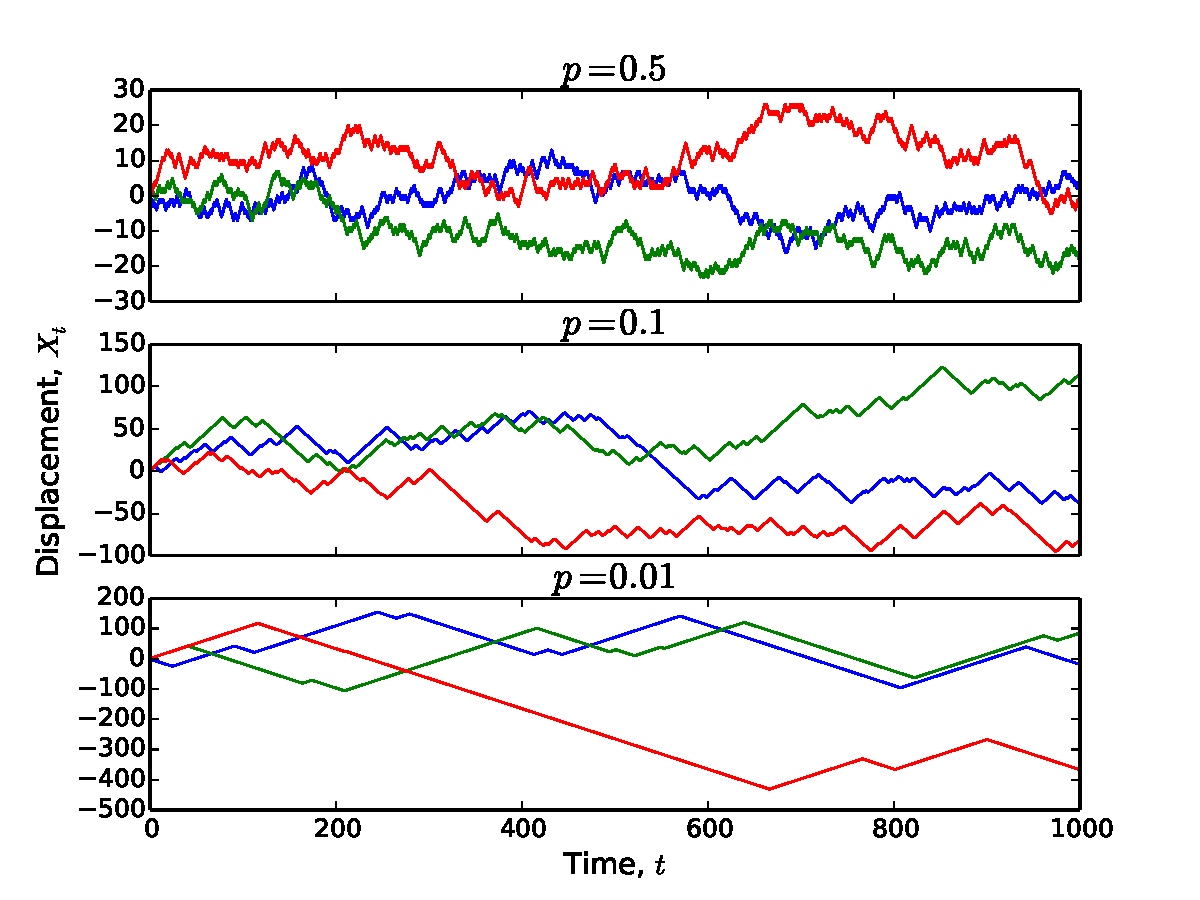
\includegraphics[width=0.95\textwidth]{small_stock.pdf}
\caption{Displacement as a function of number of steps taken for 3 Monte Carlo simulations of the randomwalker for different $p$-values. \label{fig:walk1}}
\end{figure}

% It could also be of interested to do a convergence test on the various $p$-values, to see how $\langle X^2 \rangle_N$ grows with $N$. By running the simulation for $N$ for many different values and comparing the growth of $\langle X^2 \rangle_N$ shows that it grows as $$\langle X^2 \rangle_N \propto N \quad \forall p.$$ 

% \begin{center}
% \begin{tabular}{|c||c|c|c|c|c|}\hline
% $p$ & $0.01$ & $0.10$ & $0.50$ & $0.9$ & $0.99$ \\ \hline \hline
% $<X^2>$ & 93732 & 9038 & 997 & 111 & 11 \\ \hline
% \end{tabular}
% \end{center}

\clearpage

\subsection*{Exercise 1.2}

We now make a log-log plot of the variance of the displacement as a function of time $\langle \Delta X^2 \rangle_t$ for $p=0.01$ and $p=0.1$. As before, the results are taken as the ensamble average of $10^5$ ensambles. The code is again shown in the appendix. The results are shown in figure \ref{fig:loglog}.

\begin{figure}[h]
\centering
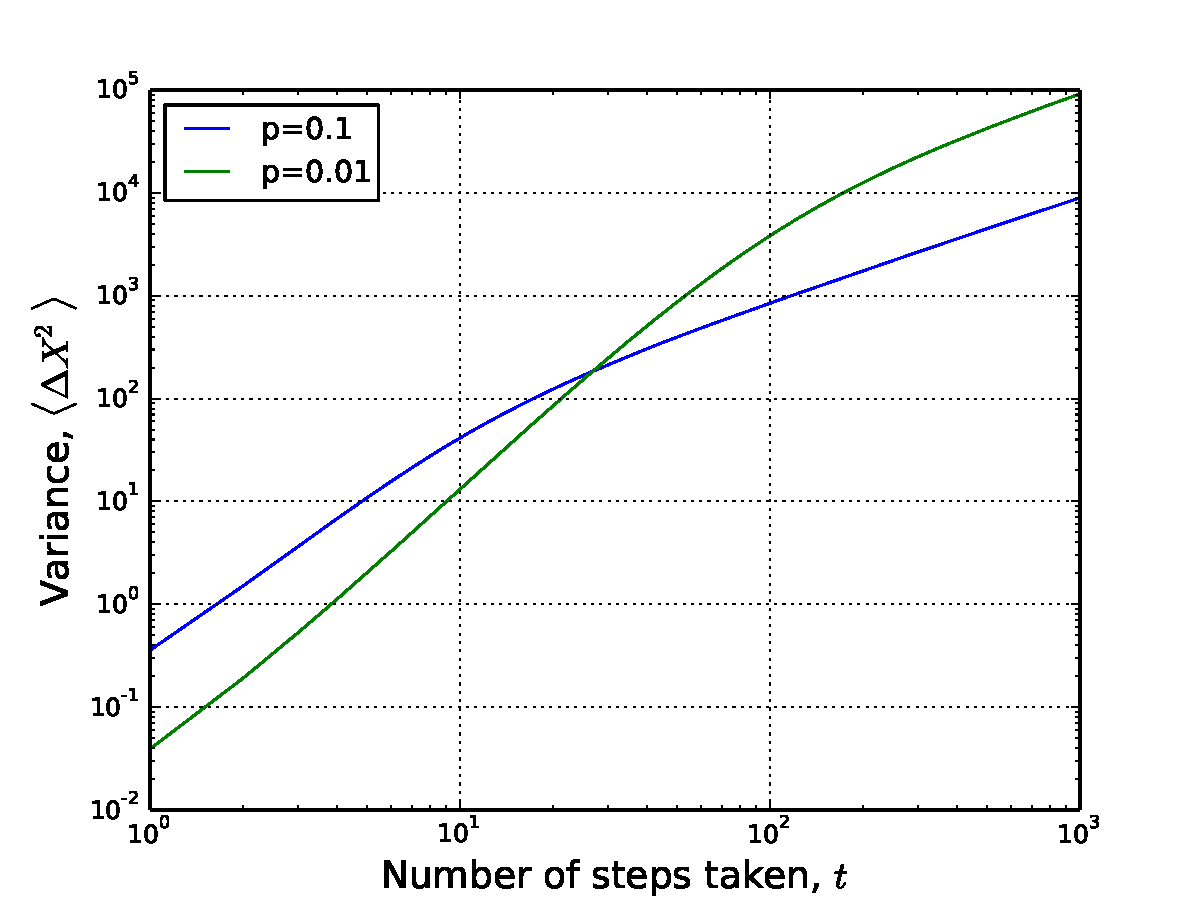
\includegraphics[width=0.75\textwidth]{loglog.pdf}
\caption{A log-log plot of the variance as a function of time for $p=0.1$ and $ p=0.01$. \label{fig:loglog}}
\end{figure}

Looking at the log-log plot, we clearly see that the variance follows some power laws as a function of time for both $p$-values, this is seen from linear portions of the curves. The slope of a linear function in a log-log plot is equal to the exponent in the power law. In both cases, we see the curves start out linear, but then change their slope gradually through some region before stabilizing again with a lower constant slope. The higher $p$-value undergoes this change in slope at an earlier time than the lower $p$-value.

The reason for the growth reducing over time is connected to the asymmetry of the walkers. Due to the initial condition of the walkers being positive, $x_0 = 1$, the $p<1/2$ walkers have a tendency of moving to the right at early times. For a symmetric walker, we require $\langle X \rangle_t = 0$, but this is definitly not the case for $x_0 = 1$ and $p < 1/2$, where $\langle X \rangle$ will be larger the smaller $p$ is.

It is the initial condition that introduces the asymmetry of the walker, as $x_1$ is $-1$ with probability $p$ and $1$ with probability $1$, which is definitly not symmetrical when $p \neq 1/2$. However, after some time $t$, the probability of $x_{i+1}$ being $1$ or $-1$ goes to 0.5, as the the system `forgets' its initial condition. We can show this through Monte Carlo simulations, we simply see what ratio of the walkers in our ensamble have $x_i = 1$. The results are shown in figure \ref{fig:system_memory}, on the next page.

From figure \ref{fig:system_memory} we clearly see the asymmetry of the $p<1/2$ walkers. The probability of taking a right step starts at $1-p$ and goes to $1/2$ over time, meaning $p=1/2$ gives a true symmetryic walker, as explained earlier. We also see that a smaller $p$ means it takes longer until the walker becomes symmetric. The time before the walker becomes symmetric is what leads to the larger early time growth in the log-log plot, as the asymmetry will enable the walkers to get away from the origin quicker. As the asymmetry dies out, the growth is reduced. In fact, looking at the time-scales, they fit very well together. For $p=0.1$ we see that the growth is reduced by $t=10^1$, which is where the asymmetry has died out in the memory plot, while for $p=0.01$ it's around $t=10^2$, which also fits the memory plot.

\begin{figure}[h]
\centering
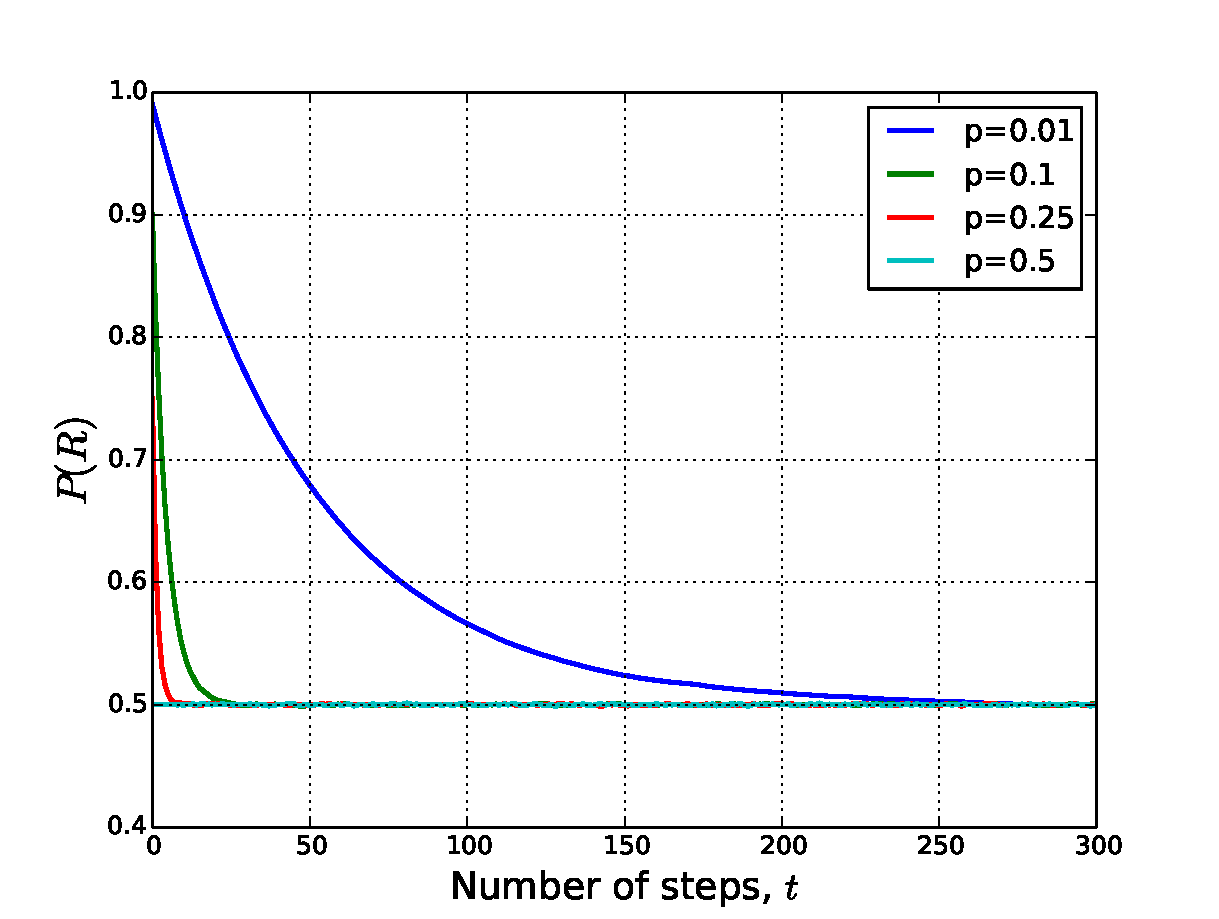
\includegraphics[width=0.75\textwidth]{memory.pdf}
\caption{The probability of a random walker taking a right step as a function of the number of steps already taken, for different values of $p$. The results are generated using a Monte Carlo simulation averaged over $10^6$ ensambles. \label{fig:system_memory}}
\end{figure}

\subsection*{Exercise 1.3}
We will now find the variance as a function of time analytically for the symmetric $p=1/2$ walker. For this walker, we now that the increment $x_i$ is positive with probability 1/2 and negative with probability $1/2$. So the position of the walker grows as
$$X_{i+1} = X_{i} \pm 1,$$
where the `$\pm$' refers to the different steps. From this, we easily find how the expectancy of the displacement grows
$$\langle X \rangle_{i+1} = \langle X \rangle_i + \frac{1}{2} - \frac{1}{2} = \langle X \rangle_i$$
So from the fact that $X_0 = 0$, we see that $\langle X \rangle_t = 0.$ By squaring the equation,
$$X_{i+1}^2 = X_{i}^2 \pm 2X_{i} + 1,$$
we can also find how the expectancy of the squared displacement grows
$$\langle X_{i+1}^2 \rangle = \langle X_{i}^2 \rangle + 1,$$
and so from $X^2_0 = 0$ we get $\langle X^2\rangle_t = t$.

The variance at time $t$ is then
$$\langle \Delta X^2 \rangle_t = \langle X^2 \rangle_t - \langle X \rangle_t^2 = t.$$
Which we may write as
$$\langle \Delta X^2 \rangle_t = 2Dt,$$
for $D=1/2$. 

\clearpage

\subsection*{Exercise 1.4}

We now let $X(t)$ represent the position of a molecule in a gas, and try to interpret what the parameter $p$ represents. For a low $p$ the molecule will rarely change direction and will tend to move in a given direction for several steps before turning, while for a high $p$ the molecule will change direction very often. The reason a molecule in a gas would change direction is because it collides with another molecule in the gas. Thus $p$ is the probability of the molecule colliding with another molecule in the gas on the time scale of a time step.

It is very reasonable to assume that the probability of collisions between the molecules is proportional to the density of the gas, as we would expect more frequent collisions in a dense gas. The molecule size will of course play a role in what $p$ is a reasonable choice for a given gas at a given density.

A very low $p$ thusly represents a gas where there are very few collisions, it could therefore be reasonable to say that a gas with a very small $p$-value can be approximated as an ideal gas.

In the reverse case, when $p \to 1$ the gas becomes very dense, and for $p = 1$, the molecule only vibrates back and forth around some equilibrium position, i.e., we have approximated a solid where the molecules are stuck in their lattice coordinates.

\subsection*{Exercise 1.5}

We now want to find the distribution of $X_N$, i.e., $P(X)_N$. We do this only for $N=1000$. To do this, we again do a monte carlo simulation for an ensamble of walkers for a given $p$-value. But instead of just looking at the ensamble average, we now plot all the ensamble results as a histogram. We then fit a normal distribution to the results, as it is reasonable to assume the results will be normally distributed due to the central limit theorem. We find a gaussian fit for $p=0.5$ and $p=0.9$.

The simple histograms of $P(X)_{1000}$ for $p=0.5$ and $p=0.9$ are shown in figure \ref{fig:hist05} and \ref{fig:hist09} respectively. In both figures, we see the results seem to be normally distributed. And the fit with the ensamble average for the mean and the standard deviation is shown.

\begin{minipage}{\linewidth}
      \centering
      \begin{minipage}{0.45\linewidth}
          \begin{figure}[H]
              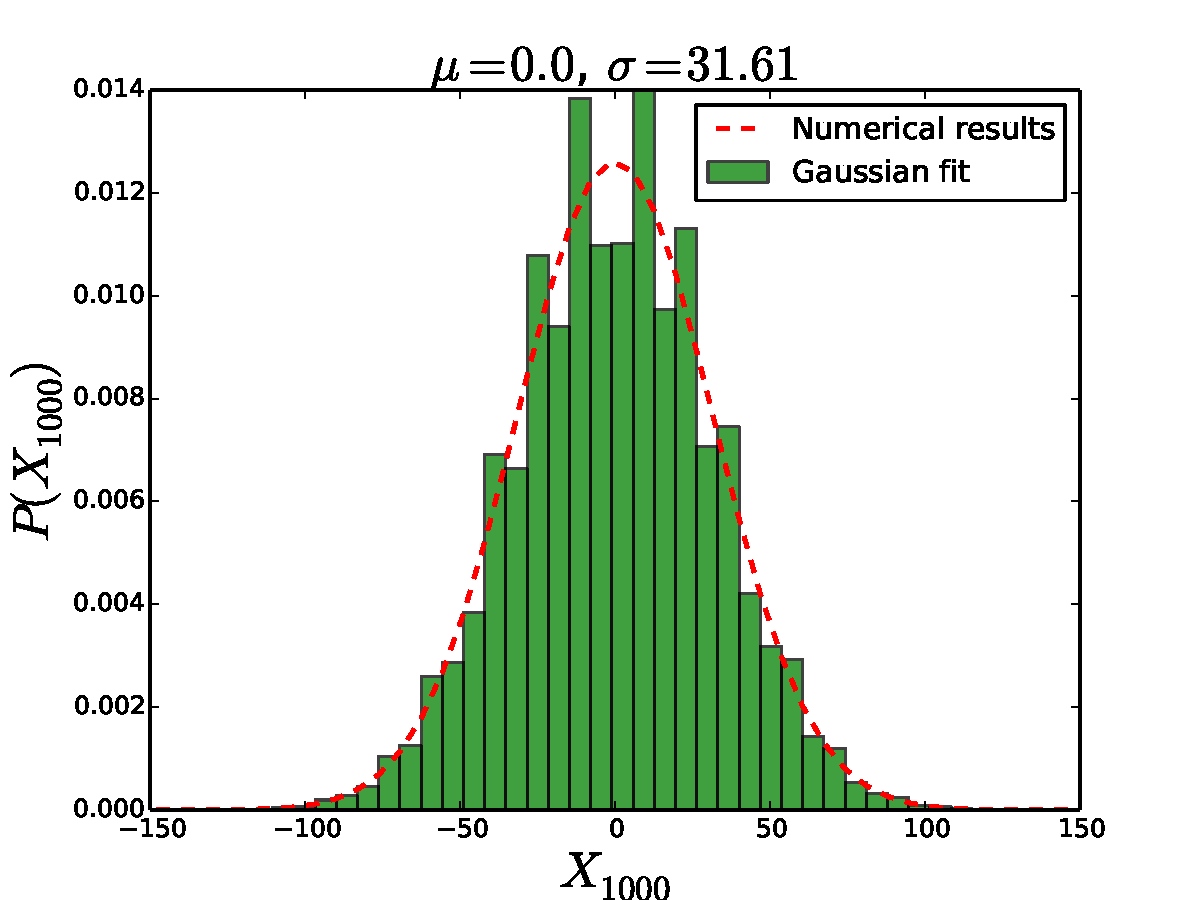
\includegraphics[width=\linewidth]{simple_hist3}
              \caption{Histogram of ensamble results for $p=0.5$, with $10^7$ ensambles. \label{fig:hist05}}
          \end{figure}
      \end{minipage}
      \hspace{0.05\linewidth}
      \begin{minipage}{0.45\linewidth}
          \begin{figure}[H]
              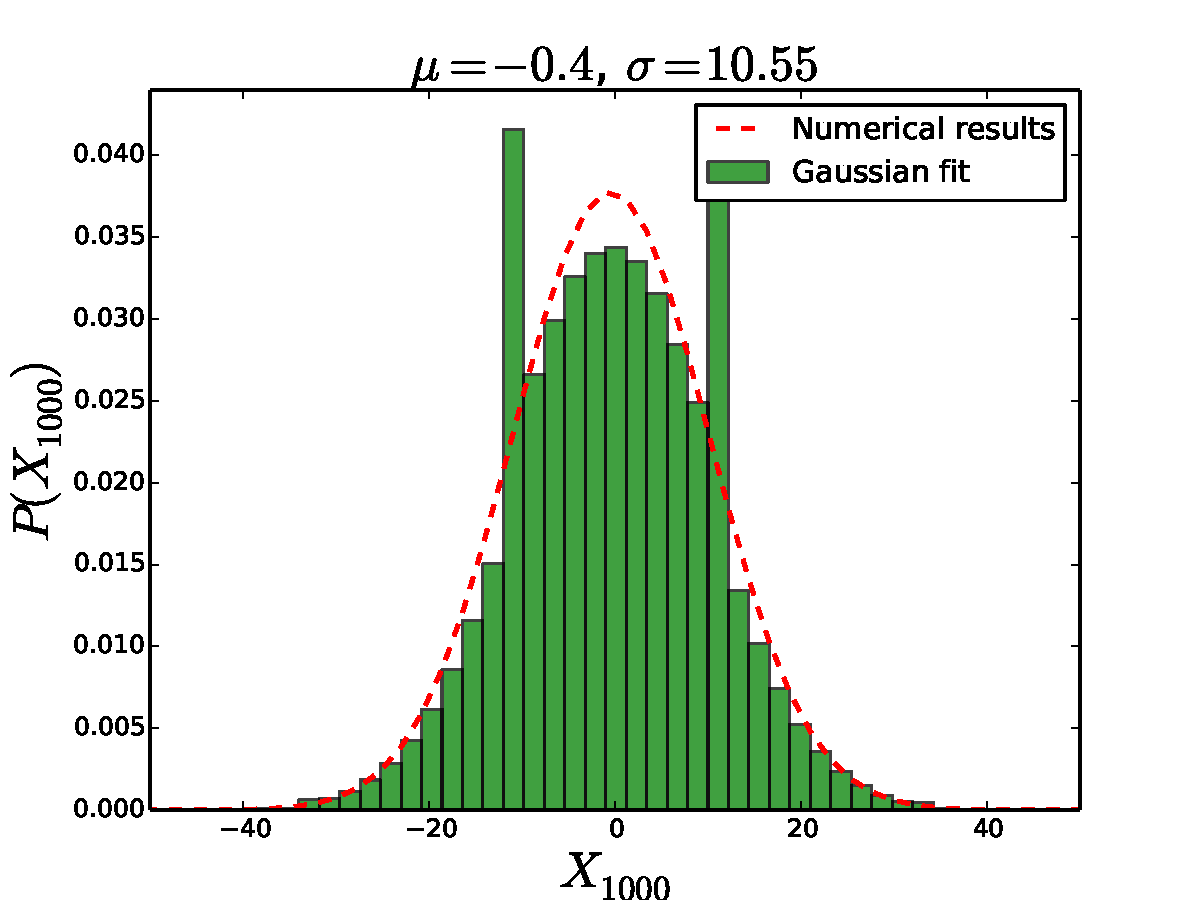
\includegraphics[width=\linewidth]{simple_hist4}
              \caption{Histogram of ensamble results for $p=0.9$, with $10^7$ ensambles. \label{fig:hist09}}
          \end{figure}
      \end{minipage}
  \end{minipage}

\clearpage

A normal distribution is defined as
$$f(x, \mu, \sigma) = \frac{1}{\sigma\sqrt{2\pi}}\exp\bigg(-\frac{(x-\mu)^2}{2\sigma^2}\bigg).$$

We can estimate $\mu$ and $\sigma$ from our ensamble average and standard deviations. The results of these estimations were shown in figure \ref{fig:hist05} and \ref{fig:hist09} and they were

\begin{table}[h!tpb]
\begin{center}
\begin{tabular}{|c|c|c|}
\hline
$p$  & $\mu$ & $\sigma$ \\ \hline 
0.5 & 0.0 & 31.6 \\ \hline
0.9 & -0.4 & 10.55 \\ \hline
\end{tabular}
\caption{Estimated parameters for the normal distributions of $P(X)_{1000}$.}
\end{center}
\end{table}

Using the estimated parameters, the distributions of $P(X_{1000})$ for $p=0.5$ and $p=0.9$ are
$$P(X)_{1000}^{p=0.5} = 0.0126\exp\bigg(-\frac{x^2}{1997}\bigg).$$
$$P(X)_{1000}^{p=0.9} = 0.0378\exp\bigg(-\frac{(x+0.4)^2}{223}\bigg).$$

For $p=0.5$ we see that this is very reasonable, as the symmetrical walker has $\langle X \rangle = 0$ and $\langle X^2 \rangle = N$, so the known analytical solution is $\mu =0$ and $\sigma = \sqrt{1000} \approx 31.62$. For $p=0.9$, we see that $\mu < 0$, which makes sense as the initial condition leads to an asymmetrical walker that has a stronger likelihood of stepping left for small times, as the time gets larger, the walker becomes symmetrical. We also note that the standard deviation is significantly smaller for $p=0.9$ than for $p=0.5$, which is also as expected, as the $p=0.9$ tends to change direction very often and so will not get as far away from the origin.

If we were to plot $\ln(P(X))$ against $X^2$ we would get a straight line decreasing with slope $a$, which would be given by 
$$a = \frac{1}{2\sigma^2}.$$

\clearpage

\section*{Exercise 1.6}
To calculate $\langle X^2(t) \rangle$ we have use the integral
$$\langle X^2(t) \rangle = \int_{-\infty}^\infty X^2 P(X)_t \ \d X.$$
The normal distribution, $f(x,\mu,\sigma)$ is normalized for any $\mu$ and $\sigma$ and so there is no need to divide by $\int_{-\infty}^\infty P(X) \ \d x = 1$.

Using our estimation of the distributions as $t=1000$, we can now calculate the expectancy of the squared displacement at this time
$$\langle X^2 \rangle_{1000} = \int_{-\infty}^\infty X^2 P(X)_{1000} \ \d X.$$

Let us calculate $\langle x^2\rangle$ for a general normal distribution
$$\frac{1}{\sqrt{2\pi}\sigma}\int_{-\infty}^\infty x^2 \exp\bigg(-\frac{(x-\mu)^2}{2\sigma^2}\bigg).$$
substituting $y=x-\mu$ gives
\begin{align*}
\langle x^2 \rangle &= \frac{1}{\sqrt{2\pi}\sigma}\bigg[\int_{-\infty}^\infty y^2 \exp\bigg(-\frac{(x-\mu)^2}{2\sigma^2}\bigg) \ \d x \\ &\qquad\qquad + 2\mu \int_{-\infty}^\infty  y \exp\bigg(-\frac{(x-\mu)^2}{2\sigma^2}\bigg) \ \d x \\&\qquad\qquad\qquad\qquad+ \mu^2 \int_{-\infty}^\infty \exp\bigg(-\frac{(x-\mu)^2}{2\sigma^2}\bigg) \ \d x\bigg].	
\end{align*}
From Rottmann p.\ 155, we see that
$$\int_{-\infty}^\infty x^2 e^{-ax^2} = \begin{cases}
	\sqrt{2\pi\sigma^2} & \mbox{for } p = 0, 1 \\
	\sqrt{2\pi\sigma^2}\sigma^2 & \mbox{for } p = 2.
\end{cases}$$
So we get
\begin{align*}
\langle x^2 \rangle &= \frac{1}{\sqrt{2\pi}\sigma}\bigg[\sqrt{2\pi\sigma^2}\bigg(\sigma^2 + 2\mu + \mu^2\bigg)\bigg] = \sigma^2 + 2\mu + \mu^2.	
\end{align*}

Now let us use this result to calculate the expectancy of the displacement squared at $t=1000$ for $p=0.5$ and $p=0.9$. First, for $p=0.5$ we get
$$\langle X^2\rangle_{1000}^{p=0.5} = 31.6^2 = 999.$$
And for $p=0.9$ we get
$$\langle X^2\rangle_{1000}^{p=0.9} = 10.55^2 + 2\cdot(-0.4) + (-0.4)^2 = 111.$$
So we see that the expectancy for the squared displacement is much lower for $p=0.9$, as expected.

For the $p=0.5$, we know that $\mu = 0$ so we have
$$\langle X^2 \rangle_{1000}^{p=0.5} = \sigma^2 = \frac{1}{2a}.$$
From exercise 1.3 we found that $\langle X^2 \rangle_{1000}^{p=0.5}$ was given by $2Dt$, so we see that
$$a = \frac{1}{4Dt}.$$

\clearpage

\section*{Exercise 2}

In this exercise we will be looking at black-body radiation in a fictional, two-dimensional world, and study how it differs from black-body radiation in our three-dimensional world.

We will assume we have periodic boundary conditions in open space, this means the field will repeat itself every length $L$ in either dimension, so we have
$$\psi(\vec{r} + L\hat{e}_i) = \psi(\vec{r}),$$
where $\hat{e}_i$ are the unit vectors in our two dimensions. From this equality, we see that the field can be described as a set of harmonic oscillators with wave numbers quantized on the form
$$k_x = \frac{2\pi n_x}{L}, \qquad k_y = \frac{2\pi n_y}{L}, \qquad n_x, n_y \in \mathbb{Z}.$$
These are different wave numbers from those we would have if we instead studied the electromagnetic field inside a box, where the wave numbers are instead $k_i = \pi n_i/L$.

The various possible wave numbers correspond to different modes of the field, and can thus be related to photons with different momenta and energies. Photons are ultrarelativistic particles, and so have energies given by
$$\eps_k = pc = \hbar c k.$$
We also know that photons are bosons, and so they must follow a Bose-Einstein distribution, using the energies we just found and the fact that $\mu=0$ for photons, we find the average number of photons in each mode of the electromagnetic field
$$\langle n_k\rangle = \frac{1}{e^{\beta\hbar c k} - 1},$$
The average energy any mode contributes to the total energy of the field is thus $\eps_k \langle n_k \rangle$, summing over all modes gives us the total energy of the field
$$U(T) = \sum_{k_x, k_y} \frac{\hbar c k}{e^{\beta \hbar c k} - 1} = \frac{2\pi}{L} \hbar c \sum_{n_x, n_y} \frac{n}{e^{2\pi/L\beta\hbar c k} - 1},$$
This expression is the first deviation from the tree-dimensional case. In the three-dimensional case, a factor of 2 has to be included, as every mode will contribute twice, as it the electromagnetic field can have two independant polarizations, which is not possible in two dimensions.

As long as the length of the periodicity of the field is large enough, the modes will be very dense and the sum will have an enormous amount of terms, so we can replace it by an integral. We write the integral in terms of polar coordinates, so we integrate over the magnitude $n$ and the angle $\theta$
$$U(T) = \frac{2\pi}{L} \hbar c \int_0^\infty \int_0^{\pi/2} \frac{n}{e^{2\pi/L\beta \hbar  c k} - 1} \ n \ \d n\  \d \theta.$$
Note that $\theta$ only goes to $\pi/2$, this is because we originally only summed $n_x$ and $n_y$ from 1 and up, this corresponds only to the first quadrant in the two-dimensional $k$-space. Also, we get an additional factor of $n$ from the Jacobian. The angular integral gives $\pi/2$ as the integrand is independant of $\theta$, so we have\footnote{Interestingly enough, the angular integral gives the exact same result in 2D as 3D, as the magnitude of the circumference of the purely positive part of the unit circle is equal to the magnitude of the purely positive surface of the unit sphere. This is however not  the case for higher-order hyperspheres. In 3D however, the Jacobian gives an additional power of $k$, and so the remaining integrands differ.}
$$U(T) = \frac{\pi^2}{L} \hbar c \int_0^\infty \frac{n^2}{e^{2\pi/L\beta \hbar  c k} - 1} \ \d n.$$

\clearpage

To carry out the final integral, it is conveniant to use the substitution
$$x = \frac{2\pi}{L}\beta\hbar c n, \qquad \d n = \frac{2\pi}{L}\beta\hbar c \ \d n,$$
which gives
$$U(T) = \frac{\pi^2}{L} \hbar c \bigg(\frac{L}{2\pi}\frac{1}{\beta \hbar c}\bigg)^3 \int_0^\infty \frac{x^2}{e^{x} - 1} \ \d x. $$
We now first expand the fraction in the integrand by $e^{-x}$ and expand the resulting denominator in a geometric series
$$U(T) = \frac{L^2}{8\pi} \frac{(kT)^3}{(\hbar c)^2} \sum_{n=1}^\infty \int_0^\infty x^2 e^{-nx} \ \d x. $$
The integral is now solvable using the definition of the $\Gamma$ function
$$U(T) = \frac{L^2}{8\pi} \frac{(kT)^3}{(\hbar c)^2} \sum_{n=1}^\infty \frac{2!}{n^{3}}$$
If we extract the numerical factor, the resulting sum is the definition of the zeta-function, so we have
$$U(T) = \frac{L^2}{4\pi} \frac{(kT)^3}{(\hbar c)^2} \zeta(3)$$

Dividing by the volume $V=L^2$ gives us the energy density, which allows us to compare to the tree-dimensional energy density
$$\mathcal{E} = \frac{U}{V} = \frac{\zeta(3)}{4\pi} \frac{(kT)^3}{(\hbar c)^2} = \frac{\zeta(3)}{4\pi}\frac{k_b^3}{(\hbar c)^2} T^3.$$
So we see that the energy density is proportional to the temperature cubed, instead of to the fourth power, which is the case in three dimensions. Also, the radiative constant is missing a factor $k_b/(\hbar c)$, as well as a having a different numerical constant in front.

We can now easily find the heat capacity at constant volume for the field
$$C_V = \bigg(\frac{\p U}{\p T}\bigg)_V = \frac{3\zeta(3)}{4\pi}\frac{k_b^3}{(\hbar c)^2} VT^2.$$






\clearpage

\section*{Appendix A---Code}

The code for all exercises was written in python.


\begin{lstlisting}
# Exercise 1.1, calculating <X^2> 

from pylab import *

N = 1000
ensambles = 1e5

def walk(p):
	X = zeros(ensambles)
	xi = ones(ensambles)

	for i in range(N):
		xi *= 2*(rand(ensambles) > p) - 1
		X += xi

	print sum(X**2)/ensambles

for p in 0.5, 0.1, 0.01:
	walk(p)
\end{lstlisting}

\begin{lstlisting}
# Exercise 1.2, calculating Var(X) plotting in a log-log plot

N = 1000
ensambles = 1e5

def plotvar(p):
	X = zeros(ensambles)
	xi = ones(ensambles)
	varX = zeros(N)

	for i in range(N):
		print i
		xi *= 2*(rand(ensambles) > p) - 1
		X += xi

		varX[i] = var(X)

	loglog(range(1, N+1), varX)

for p in 0.1, 0.01:
	plotvar(p)
\end{lstlisting}

\begin{lstlisting}
# Exercise 1.5. Make histogram of X_1000 and fit to gaussian function

from pylab import *

N = 1000
ensambles = 1e7

def hist_and_fit(p):
	X = zeros(ensambles)
	xi = ones(ensambles)

	for i in range(N):
		print i
		xi *= 2*(rand(ensambles) > p) - 1
		X += xi

	mu = mean(X)
	sigma = std(X)
	n, bins, patches = plt.hist(X, 50, normed=1, facecolor='green', alpha=0.75)
	plot(bins, normpdf(bins, mu, sigma), 'r--', linewidth=2.0)
	
	return mu, sigma

X = walk_hist(0.5)
\end{lstlisting}



\end{document}